\problemname{Tiles}

Karin has invented a solitaire game played with Othello tiles, which are
black on one side and white on the other side. She lays out a row of
tiles, each of which can be black or white. The goal is to make all tiles have the white side up.

A ``move'' is to ``pick out'' an adjacent pair of tiles
somewhere from the sequence, flip them (white becomes black, black becomes
white), and put them back either at the beginning of the row or at the end of
the row, without changing the pair's internal order.

Write a program that, given the original row of tiles,
outputs the minimum number of moves needed to
make all tiles white.

\begin{center}
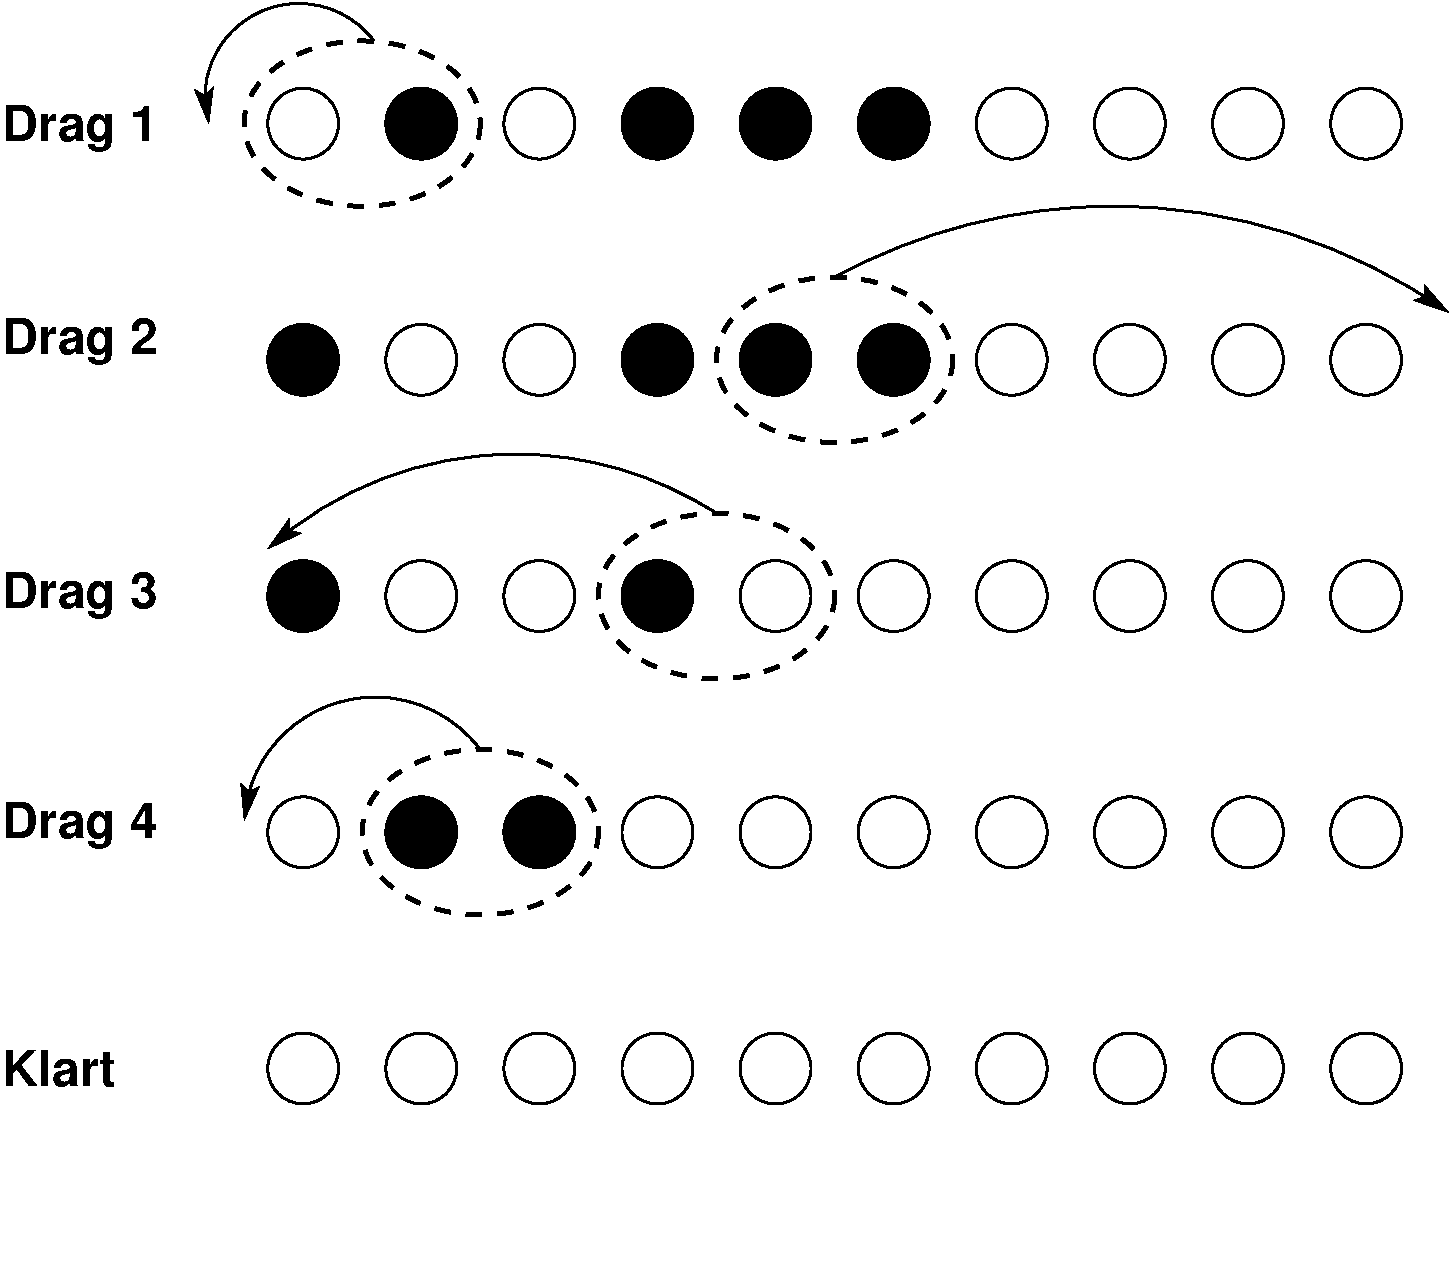
\includegraphics[width=12cm]{brickorbild.pdf}\\
{\em A possible move sequence in sample 2}
\end{center}

\section*{Input}

The input consists of a string containing only the letters \texttt S and \texttt V.
The string is between 3 and 15 characters long.

\section*{Output}

Output a single number: the minimum number of moves needed to
make all tiles white. For the given test data, it will always be
possible to reach the goal.

\section*{Scoring}
For test cases worth $60$ points, the string length is at most 10 and the answer is at most 6.\\
For test cases worth $40$ points, no special constraints apply.
